% Options for packages loaded elsewhere
\PassOptionsToPackage{unicode}{hyperref}
\PassOptionsToPackage{hyphens}{url}
%
\documentclass[
]{article}
\usepackage{lmodern}
\usepackage{amsmath}
\usepackage{ifxetex,ifluatex}
\ifnum 0\ifxetex 1\fi\ifluatex 1\fi=0 % if pdftex
  \usepackage[T1]{fontenc}
  \usepackage[utf8]{inputenc}
  \usepackage{textcomp} % provide euro and other symbols
  \usepackage{amssymb}
\else % if luatex or xetex
  \usepackage{unicode-math}
  \defaultfontfeatures{Scale=MatchLowercase}
  \defaultfontfeatures[\rmfamily]{Ligatures=TeX,Scale=1}
\fi
% Use upquote if available, for straight quotes in verbatim environments
\IfFileExists{upquote.sty}{\usepackage{upquote}}{}
\IfFileExists{microtype.sty}{% use microtype if available
  \usepackage[]{microtype}
  \UseMicrotypeSet[protrusion]{basicmath} % disable protrusion for tt fonts
}{}
\makeatletter
\@ifundefined{KOMAClassName}{% if non-KOMA class
  \IfFileExists{parskip.sty}{%
    \usepackage{parskip}
  }{% else
    \setlength{\parindent}{0pt}
    \setlength{\parskip}{6pt plus 2pt minus 1pt}}
}{% if KOMA class
  \KOMAoptions{parskip=half}}
\makeatother
\usepackage{xcolor}
\IfFileExists{xurl.sty}{\usepackage{xurl}}{} % add URL line breaks if available
\IfFileExists{bookmark.sty}{\usepackage{bookmark}}{\usepackage{hyperref}}
\hypersetup{
  hidelinks,
  pdfcreator={LaTeX via pandoc}}
\urlstyle{same} % disable monospaced font for URLs
\usepackage{graphicx}
\makeatletter
\def\maxwidth{\ifdim\Gin@nat@width>\linewidth\linewidth\else\Gin@nat@width\fi}
\def\maxheight{\ifdim\Gin@nat@height>\textheight\textheight\else\Gin@nat@height\fi}
\makeatother
% Scale images if necessary, so that they will not overflow the page
% margins by default, and it is still possible to overwrite the defaults
% using explicit options in \includegraphics[width, height, ...]{}
\setkeys{Gin}{width=\maxwidth,height=\maxheight,keepaspectratio}
% Set default figure placement to htbp
\makeatletter
\def\fps@figure{htbp}
\makeatother
\setlength{\emergencystretch}{3em} % prevent overfull lines
\providecommand{\tightlist}{%
  \setlength{\itemsep}{0pt}\setlength{\parskip}{0pt}}
\setcounter{secnumdepth}{-\maxdimen} % remove section numbering
\ifluatex
  \usepackage{selnolig}  % disable illegal ligatures
\fi

\author{}
\date{}

\begin{document}

\hypertarget{header-n0}{%
\subsection{Documents \& Data on the Web Coursework}\label{header-n0}}

\begin{quote}
\textbf{Name}: weilue luo\\
\textbf{ID}: 10404762\\
\textbf{Date}: 16 Nov 2020
\end{quote}

\tableofcontents

\hypertarget{header-n7}{%
\subsection{Preface}\label{header-n7}}

I am using intellij with Java 8. Note that there are more technical
explanations in the code. Note that I put many utilities functions /
classes into the BasicInvertedIndex file, this is bad practice, but
according to instruction I can only submit this class' file.

\hypertarget{header-n9}{%
\subsection{Functionality}\label{header-n9}}

\hypertarget{header-n10}{%
\subsubsection{Features, Improvements \& Problems}\label{header-n10}}

\hypertarget{header-n426}{%
\paragraph{Stream}\label{header-n426}}

Highly readable, efficient, pipelined code using the Stream API from
Java 8.

\hypertarget{header-n15}{%
\paragraph{Raw Tokenize}\label{header-n15}}

It splits text to lines by:

\begin{itemize}
\item
  Any tab, carriage-return, newline, form-feed, double-quote, and
  single-quote.
\item
  Any dot, question mark, exclamation mark that follows by
  space/tab/carriage-return/form-feed/newline.
\end{itemize}

I included quotes because they are common for quoting. Dot/Question
mark/Exclamation mark must follow by delimiter for more precise match of
end-of-sentence, e.g. it will not split statements like:
\(10.0\times 10!=\lambda\).

While it generate more suitable index term, it assumes usage of quotes
which may not be true. Moreover, the tokenization is design for English,
separators of other languages are not considered.

\hypertarget{header-n23}{%
\paragraph{Tokenize From Line}\label{header-n23}}

It cleans the word and returns true if only the first letter is
uppercase, making it more precise.

\hypertarget{header-n33}{%
\paragraph{Expand Tokens}\label{header-n33}}

A consideration on multi-term/single term:

\begin{itemize}
\item
  \textbf{Number}: keep original token because user may search using it.
\item
  \textbf{Date}: Keep both original token and numeric form, because user
  may just enter number without separator to search for dates.
\item
  \textbf{URL}: Break it into pieces by punctuations, because the user
  may not search the full URL.
\item
  \textbf{Connected Word}: Keep each pieces as well, e.g. ease-of-access
  \(\rightarrow\) {[}ease, of, access, easeofaccess, EOA{]}.
\item
  \textbf{Other}: Keep letters only (which is not good for other
  languages).
\end{itemize}

All tokens share the same position to ensure it reflects the actual
position. This process may also generate blank token, but it will be
removed in latter stage. Normally, letters-only tokens are added for
more robust indexing terms.

\hypertarget{header-n48}{%
\paragraph{Stem \& Stopword Removal}\label{header-n48}}

Lemmatization and stopwords removal are achieve with stemming and
StopAnalyser, it collapse like-terms into one which make it more
suitable for indexing, however, it may introduce over-stemming problem
since it is a crude process.

\hypertarget{header-n50}{%
\paragraph{Grouping \& Reducing}\label{header-n50}}

\begin{itemize}
\item
  Used Set for positions, collapsing same expanded terms.
\item
  Note the size of positions is term frequency.
\end{itemize}

\hypertarget{header-n69}{%
\paragraph{Sorting}\label{header-n69}}

Each inverted-index is sorted using simple heuristic.

\[\text{ranking}=\text{tfidf}+\frac{\sqrt{\sigma+\lambda}}{\sigma+\lambda}\]

where \(\sigma\) is the variance of the positions and \(\lambda\) is a
constant to reduce score for low-occurrence-words.

\begin{itemize}
\item
  Not using standard-deviation because variance gives smoother step.
\item
  I used \(\lambda=20\) to dampen effect of single occurrence term and
  avoid division by zero.
\end{itemize}

\begin{figure}
\centering
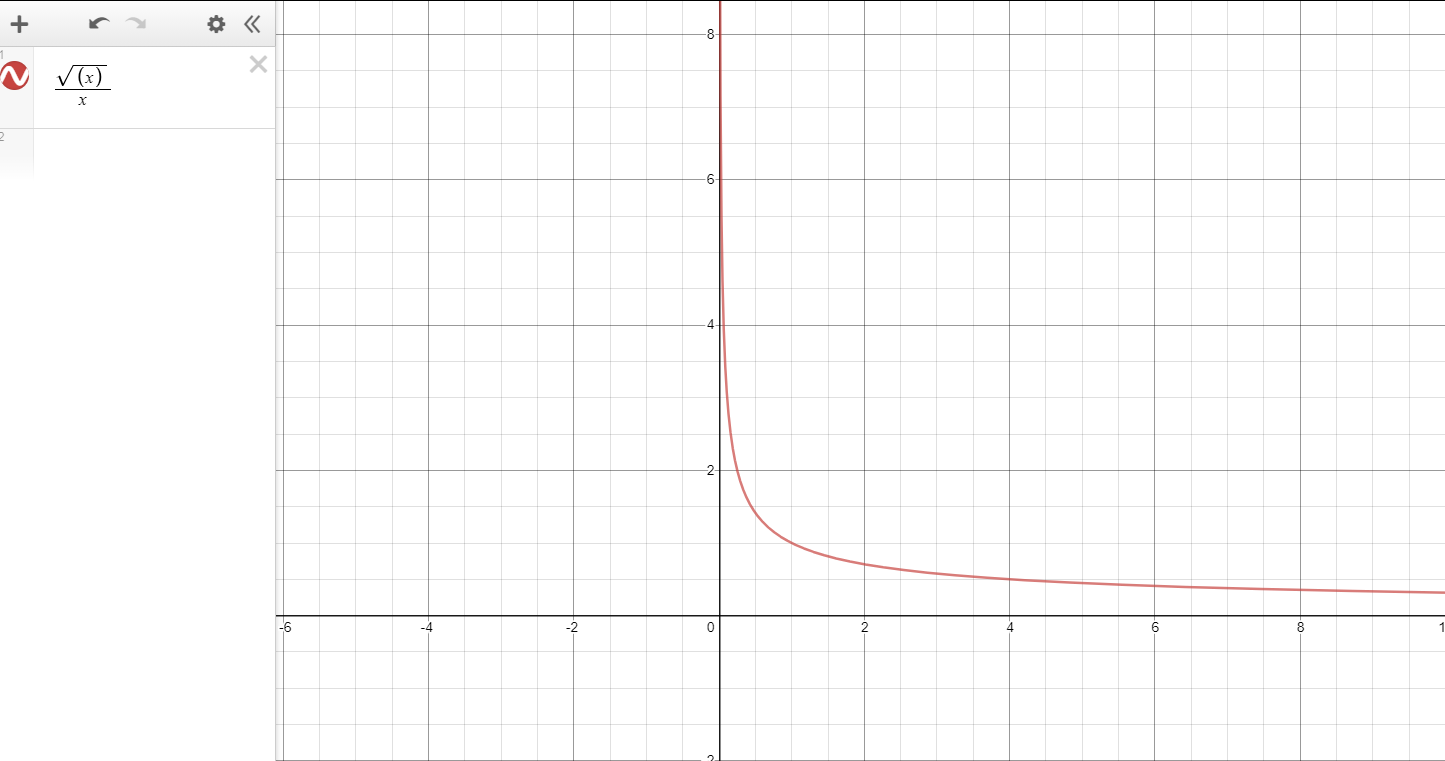
\includegraphics{D:/UOM/Projects/Notes/docs_cwk.assets/image-20201118163620038.png}
\caption{sqrtx/x}
\end{figure}

\textbf{Example A}

\begin{itemize}
\item
  \textbf{TFIDF}

  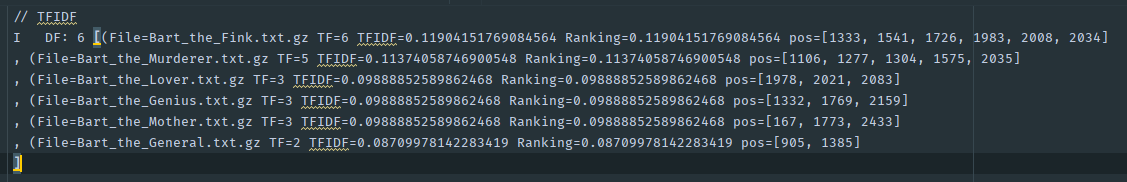
\includegraphics{D:/UOM/Projects/Notes/docs_cwk.assets/image-20201118154329554.png}\\
  Although \emph{Bart\emph{the}lover} has less occurrence of the token
  "I", it is arguably better than \emph{Bart\emph{the}Murderer} because
  those three words have very low variance, therefore the variance is
  getting too little weight this case.
\item
  \textbf{My heuristic (Standard Deviation)}

  \begin{figure}
  \centering
  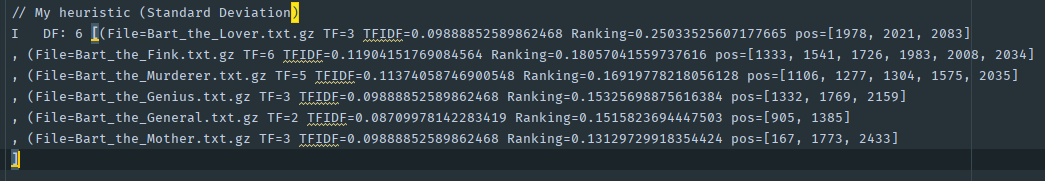
\includegraphics{D:/UOM/Projects/Notes/docs_cwk.assets/image-20201118154523202.png}
  \caption{}
  \end{figure}

  By using standard deviation heuristic, \emph{Bart\emph{the}lover}
  raised to the first place, but clearly this is over-done, because
  although \emph{Bart\emph{the}Fink} has higher variance overall, it has
  low variance with positions: 1983, 2008 and 2034, therefore the
  variance is getting too much weighting in this case.
\item
  \textbf{My heuristic (Variance)}

  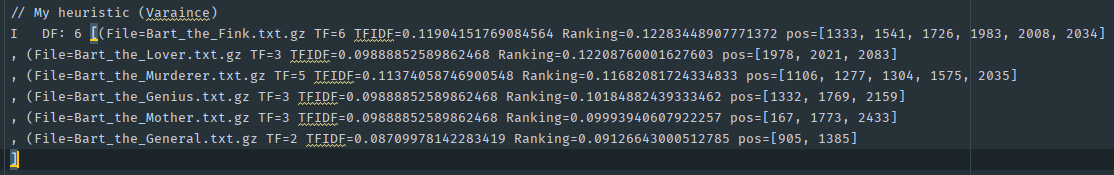
\includegraphics{D:/UOM/Projects/Notes/docs_cwk.assets/image-20201118154648301.png}\\
  By using variance heuristic, \emph{Bart\emph{the}Lover} got the right
  position, thus this heuristic is most suitable among three variance.
\end{itemize}

Note that this heuristic does not work well for some cases, e.g.:

\begin{itemize}
\item
  Single occurrence term, because it has 0 variance which made it score
  very high.

  \begin{itemize}
  \item
    One way to dampen this effect is to assign a slightly higher
    \(\lambda\), but it does not solve the problem.
  \item
    A better options would be make use of the number of positions.
  \end{itemize}
\item
  Very short documents, the step of the \(\frac{\sqrt{\sigma}}{\sigma}\)
  will be very steep which made it very sensitive to variance, resulting
  in overly high difference.
\end{itemize}

\hypertarget{header-n77}{%
\subsubsection{Other Limitations}\label{header-n77}}

\begin{itemize}
\item
  Lack of language support, it will not work against other language such
  as Japanese.
\item
  Lack of document type support, it assumes the input are plain text,
  and does not check for images, file formats, video, etc.
\item
  The current handling of special tokens are not robust enough, it
  merely handles:

  \begin{itemize}
  \item
    Numeric token.
  \item
    Simple date-like token.
  \item
    URL token.
  \item
    dash-connected multi-term.
  \end{itemize}

  Some unhandled token includes: measures, citations, hashtags, etc.
\item
  It does not check for spelling in the documents and assume it is
  correct, however, this should be fine for most cases.
\item
  The output of MapReduce is sorted alphabetically which is not very
  helpful. For this we have to write our own partitioner which is not
  trivial.
\end{itemize}

\hypertarget{header-n101}{%
\subsection{Performance}\label{header-n101}}

\hypertarget{header-n102}{%
\subsubsection{Design Patterns \& Effects}\label{header-n102}}

The overall design pattern is Map \& Reduce, which is optimized for
distributed computing. Obviously, this slows down performance since we
only have one computer with little data, but for the purpose of
coursework it is fine.

I made heavy use of Java 8's features such as Stream, lambda expression,
method references, etc to chain my operations to achieve high
efficiency. It is possible to squeeze everything into some
while/for-loop, it generally gives slightly better performance, but I
think readability is more important than minor performance loss.

\hypertarget{header-n104}{%
\paragraph{Positional TF Term}\label{header-n104}}

This is a class used to group all relevant data for a term, and provide
useful utilities such as merging. It follows the immutability and
factory design pattern which made it much safer and easier to use.

\hypertarget{header-n308}{%
\paragraph{In-mapper Aggregation}\label{header-n308}}

I lifting most of the reducer's tasks by using groupingBy and reducing
code in the mapper, all reducer does is directly output the given
Iterable\textless{}PositionalTFTerm\textgreater{}, after some
calculations (TFIDF and ranking) and converting it to a writable array.

\hypertarget{header-n327}{%
\paragraph{Stopword Removal}\label{header-n327}}

I used Set instead of List in StopAnalyser for faster stopwords checks.

\hypertarget{header-n442}{%
\paragraph{Mapper \& Reducer}\label{header-n442}}

An simple profile analysis using Java Flight Recorder revealed that map
and reduce function took 15.4\% and 3.8\% respectively and the overall
runtime is 4.52s.

\begin{figure}
\centering

\includegraphics{D:/UOM/Projects/Notes/docs_cwk.assets/image-20201118205725088.png}
\caption{}
\end{figure}

\begin{figure}
\centering

\includegraphics{D:/UOM/Projects/Notes/docs_cwk.assets/image-20201118205857852.png}
\caption{}
\end{figure}

Without mapper aggregation, the map and reduce function took 16.3\% and
11.6\% respectively and the overall runtime is 10.011s.

\begin{figure}
\centering

\includegraphics{D:/UOM/Projects/Notes/docs_cwk.assets/image-20201118213331428.png}
\caption{}
\end{figure}

\begin{figure}
\centering

\includegraphics{D:/UOM/Projects/Notes/docs_cwk.assets/image-20201118213210884.png}
\caption{}
\end{figure}

From above we see how in-mapper aggregation has significant impact on
the performance.

\hypertarget{header-n106}{%
\subsubsection{Limitations}\label{header-n106}}

\hypertarget{header-n107}{%
\paragraph{Map Reduce}\label{header-n107}}

\begin{itemize}
\item
  Reduce/Sorting is take very long time if map stage generate too many
  keys.
\item
  It is built for batch processing so not useful for interactive job.
\item
  It is not suitable for tasks that have dependency on each other since
  they cannot be parallelize.
\end{itemize}

\hypertarget{header-n108}{%
\subsection{Appendix}\label{header-n108}}

\hypertarget{header-n116}{%
\paragraph{50 lines output (1700 words)}\label{header-n116}}

\end{document}
